\section{Design}
This section describes the design of the SRI, how the tool is built, and what to look out for.
\subsection{Decision for a new Tool}
At the beginning it was not clear how the tool should be built exactly and what the functionality and scope should be based on. After a detailed analysis of different tools, reports and studies, it was possible to better estimate how an efficient detection of the readiness of a system can be implemented. It would have been desirable to be able to build on an existing tool, but as shown in a five-week analysis, there is no such tool. For this reason it was decided to develop a tool based on JPCERT/CCs study. The configurations in the Advanced Audit Settings of the GPOs are to be checked accordingly and in a second step the event logs are to be searched for the EventIDs.

\subsection{Mandatory Event Logs}\label{MandatoryLogs}
The following tables lists the event logs which are mandatory and must be logged based on the study ''\nameref{JPCertStudy}'':
\
\vspace{0.5cm}
\begin{table}[H]
    \centering
    \begin{tabular}{| p{1.5cm} | p{14.5cm} |} \hline
        \multicolumn{2} {|c|} {\tiny\bfseries System} \\ \hline
        \textbf{EventID} & \textbf{Description}  \\ \hline
        8222\footnotemark[2] & Shadow copy has been created \\ \hline
        20001\footnotemark[2] & Driver Management concluded the process to install driver  \\ \hline
    \end{tabular}
    \caption{Mandatory System Event Logs}
\end{table}
\footnotetext[2]{Recorded by default Windows settings}


\begin{table}[H]
    \centering
    \begin{tabular}{| p{1.5cm} | p{14.5cm} |} \hline
        \multicolumn{2} {|c|} {\tiny\bfseries Applications \& Service > Microsoft > Windows > TaskScheduler > Operational} \\ \hline
        \textbf{EventID} & \textbf{Description}  \\ \hline
        102\footnotemark[2] & Task completed \\ \hline
        106\footnotemark[2] & A task has been registered \\ \hline
        129\footnotemark[2] & A task process has been created \\ \hline
        200\footnotemark[2] & The operation that has been started \\ \hline
        201\footnotemark[2] & The operation has been completed \\ \hline
    \end{tabular}
    \caption{Mandatory TaskScheduler Event Logs}
\end{table}

\begin{table}[H]
    \centering
    \begin{tabular}{| p{1.5cm} | p{14.5cm} |} \hline
        \multicolumn{2} {|c|} {\tiny\bfseries Applications \& Service > Microsoft > Windows > Windows Remote Management > Operational} \\ \hline
        \textbf{EventID} & \textbf{Description}  \\ \hline
        6\footnotemark[2] & Creating WSMan Session \\ \hline
        169\footnotemark[2] & User authentication authenticated successfully \\ \hline
    \end{tabular}
    \caption{Mandatory Windows Remote Management Event Logs}
\end{table}

\begin{table}[H]
    \centering
    \begin{tabular}{| p{1.5cm} | p{14.5cm} |} \hline
        \multicolumn{2} {|c|} {\tiny\bfseries Applications \& Service > Microsoft > Windows > TerminalServices-LocalSessionManager > Operational} \\ \hline
        \textbf{EventID} & \textbf{Description}  \\ \hline
        21\footnotemark[2] & Remote Desktop Services: Session logon succeeded\\ \hline
        24\footnotemark[2] & Remote Desktop Services: Session has been disconnected \\ \hline
    \end{tabular}
    \caption{Mandatory TerminalServices-LocalSessionManager Event Logs}
\end{table}

\begin{table}[H]
    \centering
    \begin{tabular}{| p{1.5cm} | p{14.5cm} |} \hline
        \multicolumn{2} {|c|} {\tiny\bfseries Applications \& Service > Microsoft > Windows > Sysmon > Operational} \\ \hline
        \textbf{EventID} & \textbf{Description}  \\ \hline
        1\footnotemark[3] & Process create \\ \hline
        2\footnotemark[3] & A process changed a file creation time \\ \hline
        5\footnotemark[3] & Process terminated \\ \hline
        8\footnotemark[3] & CreateRemoteThread \\ \hline
        9\footnotemark[3] & RawAccessRead: detects when the process is using ''\textbackslash\textbackslash.\textbackslash'' \\ \hline
    \end{tabular}
    \caption{Mandatory Sysmon Event Logs}
\end{table}
\nocite{Sysmon-Presentation}

\begin{table}[H]
    \centering
    \begin{tabular}{| p{1.5cm} | p{14.5cm} |} \hline
        \multicolumn{2} {|c|} {\tiny\bfseries Applications \& Service > Microsoft > Windows > TaskScheduler > Operational} \\ \hline
        \textbf{EventID} & \textbf{Description}  \\ \hline
        102\footnotemark[2] & Task completed \\ \hline
        106\footnotemark[2] & Task registered \\ \hline
        129\footnotemark[2] & Created Task Process \\ \hline
        200\footnotemark[2] & Action started \\ \hline
        201\footnotemark[2] & Action completed \\ \hline
    \end{tabular}
    \caption{Mandatory TaskScheduler Event Logs}
\end{table}

\begin{table}[H]
    \centering
    \begin{tabular}{| p{1.5cm} | p{14.5cm} |} \hline
        \multicolumn{2} {|c|} {\tiny\bfseries Applications \& Service > Microsoft > Windows > WinRM > Operational} \\ \hline
        \textbf{EventID} & \textbf{Description}  \\ \hline
        6\footnotemark[2] & Creating WSMan Session \\ \hline
        169\footnotemark[2] & User authentication: authenticated successfully \\ \hline
    \end{tabular}
    \caption{Mandatory Windows Remote Management Event Logs}
\end{table}

\begin{table}[H]
    \centering
    \begin{tabular}{| p{1.5cm} | p{14.5cm} |} \hline
        \multicolumn{2} {|c|} {\tiny\bfseries Applications \& Service > Microsoft > Windows > TerminalServices > LocalSessionManager > Operational} \\ \hline
        \textbf{EventID} & \textbf{Description}  \\ \hline
        21\footnotemark[2] & Remote Desktop Services: Session logon succeeded \\ \hline
        24\footnotemark[2] & Remote Desktop Services: Session has been disconnected \\ \hline
    \end{tabular}
    \caption{Mandatory Windows Local Session Manager Event Logs}
\end{table}

\footnotetext[2]{Recorded by default Windows settings}
\footnotetext[3]{Recorded by default Sysmon settings}

\clearpage

\
\begin{table}[H]
    \centering
    \begin{tabular}{| p{1.5cm} | p{14.5cm} |} \hline
        \multicolumn{2} {|c|} {\tiny\bfseries Security} \\ \hline
        \textbf{EventID} & \textbf{Description}  \\ \hline
        104\footnotemark[2] & The System log file was cleared \\ \hline
        4624 & An account was successfully logged on \\ \hline
        4634 & An account was logged off \\ \hline
        4648 & A logon was attempted using explicit credentials \\ \hline
        4656 & A handle to an object was requested \\ \hline
        4658 & The handle to an object was closed \\ \hline
        4660 & An object was deleted \\ \hline
        4661 & A handle to an object was requested \\ \hline
        4663 & An attempt was made to access an object \\ \hline
        4672 & Special privileges assigned to new logon \\ \hline
        4673 & A privileged service was called \\ \hline
        4688 & A new process has been created \\ \hline
        4689 & A process has exited \\ \hline
        4690 & An attempt was made to duplicate a handle to an object \\ \hline
        4720 & A user account was created \\ \hline
        4726 & A user account was deleted \\ \hline
        4728 & A member was added to a security enabled global group \\ \hline
        4729 & A member was removed from a security enabled global group \\ \hline
        4768 & A Kerberos authentication ticket (TGT) was requested \\ \hline
        4769 & A Kerberos service ticket was requested \\ \hline
        4946 & A change has been made to Windows Firewall exception list. A rule was added \\ \hline
        5140 & A network share object was accessed \\ \hline
        5142 & A network share object was added \\ \hline
        5144 & A network share object was deleted \\ \hline
        5145 & A network share object was accessed \\ \hline
        5154 & WFP has permitted an application or service to listen on a port for incoming connections \\ \hline
        5156 & WFP has allowed a connection \\ \hline
        7036\footnotemark[2] & The service state has changed \\ \hline
        7045\footnotemark[2] & A service was installed in the system \\ \hline
    \end{tabular}
    \caption{Mandatory Security Event Logs}
\end{table}
\footnotetext[2]{Recorded by default Windows settings}
\setcounter{footnote}{3}
\clearpage

\subsection{Correlation: Advanced Audit Policy Setting and Event Log IDs}\label{Correlation}
In this section, the ''Advanced Audit Policies'' required to trigger the corresponding event logs are shown in tables. Based on these tables, the ''Advanced Audit Policies'' are checked for correctness with the tool. There are several combinations of settings which can be configured:\\
\begin{multicols}{2}
    \vspace{1cm} \null 
    \begin{description}
        \item[Not Configured:] \ \\ Nothing selected
        \item[No Auditing:] \ \\ ''Configure the following audit events:''
        \item[Success (S):] \ \\ ''Success''
        \item[Failure (F):] \ \\ ''Failure''
        \item[Success and Failure (S, F):] \ \\ ''Success'' and ''Failure'' 
    \end{description}
    \vfill \null 
    \columnbreak

    \begin{figure}[H]
        \centering
        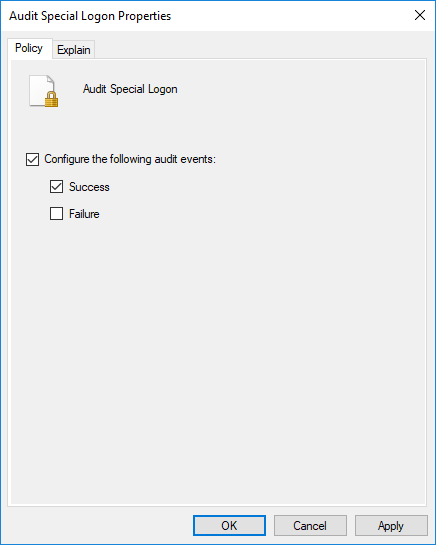
\includegraphics[width=0.75\linewidth]{assets/auditpolicies/speciallogon.png}
        \caption{Advanced Audit Policy - Logon/Logoff - Audit Special Logon}
    \end{figure}
\end{multicols}
\begin{table}[H]
    \centering
    \begin{tabular}{| p{8cm} | p{8cm} |} \hline
        \multicolumn{2} {|c|} {\tiny\bfseries Account Logon} \\ \hline
        \textbf{Subcategory} & \textbf{EventIDs}  \\ \hline
        Audit Kerberos Authentication Service & 4768(S, F) \\ \hline
        Audit Kerberos Service Ticket Operations & 4769(S, F) \\ \hline
    \end{tabular}
    \caption{Advanced Audit Policy Setting Account Logon}
\end{table}

\begin{table}[H]
    \centering
    \begin{tabular}{| p{8cm} | p{8cm} |} \hline
        \multicolumn{2} {|c|} {\tiny\bfseries Account Management} \\ \hline
        \textbf{Subcategory} & \textbf{EventIDs}  \\ \hline
        Audit User Account Management & 4720(S), 4726(S), 4738(S), 4724(S), 4722(S) \\ \hline
        Audit Security Group Management & 4728(S, F), 4729(S, F), 4737 (S, F) \\ \hline
    \end{tabular}
    \caption{Advanced Audit Policy Setting Account Management}
\end{table}

\begin{table}[H]
    \centering
    \begin{tabular}{| p{8cm} | p{8cm} |} \hline
        \multicolumn{2} {|c|} {\tiny\bfseries Detailed Tracking} \\ \hline
        \textbf{Subcategory} & \textbf{EventIDs}  \\ \hline
        Audit Process Creation & 4688(S) \\ \hline
	    Audit Process Termination & 4689(S)	 \\ \hline
    \end{tabular}
    \caption{Advanced Audit Policy Setting Logon/Logoff}
\end{table}

\begin{table}[H]
    \centering
    \begin{tabular}{| p{8cm} | p{8cm} |} \hline
        \multicolumn{2} {|c|} {\tiny\bfseries Logon/Logoff} \\ \hline
        \textbf{Subcategory} & \textbf{EventIDs}  \\ \hline
        Audit Logon & 4624(S), 4648(S)	  \\ \hline
	    Audit Logoff & 4634(S) \\ \hline
	    Audit Special Logon & 4672(S) \\ \hline
    \end{tabular}
    \caption{Advanced Audit Policy Setting Logon/Logoff}
\end{table}

\begin{table}[H]
    \centering
    \begin{tabular}{| p{8cm} | p{8cm} |} \hline
        \multicolumn{2} {|c|} {\tiny\bfseries Object Access} \\ \hline
        \textbf{Subcategory} & \textbf{EventIDs}  \\ \hline
        Audit Detailed File Share & 5145(S, F) \\ \hline		
        Audit File Share & 5140(S, F), 5142(S), 5144(S)	\\ \hline	
        Audit File System & 4656(S, F), 4658(S), 4660(S), 4663(S), 4670(S) \\ \hline
        Audit Filtering Platform Connection & 5154(S), 5156(S), 5447(S, F) \\ \hline
        Audit Handle Manipulation & 4658(S), 4690(S) \\ \hline
        Audit Kernel Object & 4656(S, F), 4658(S), 4660(S), 4663(S)	\\ \hline
        Audit Other Object Access Events & 4698(S, F) \\ \hline
        Audit Registry & 4656(S, F), 4658(S), 4660(S), 4663(S) \\ \hline
        Audit SAM & 4661(S, F) \\ \hline			
    \end{tabular}
    \caption{Advanced Audit Policy Setting Object Access}
\end{table}

\vspace{0.5cm}
\begin{table}[H]
    \centering
    \begin{tabular}{| p{8cm} | p{8cm} |} \hline
        \multicolumn{2} {|c|} {\tiny\bfseries Policy Change} \\ \hline
        \textbf{Subcategory} & \textbf{EventIDs}  \\ \hline
        Audit MPSSVC Rule-Level Policy Change &	4946(S) \\ \hline
    \end{tabular}
    \caption{Advanced Audit Policy Setting Policy Change}
\end{table}

\begin{table}[H]
    \centering
    \begin{tabular}{| p{8cm} | p{8cm} |} \hline
        \multicolumn{2} {|c|} {\tiny\bfseries Privilege Use} \\ \hline
        \textbf{Subcategory} & \textbf{EventIDs}  \\ \hline
        Audit Non Sensitive Privilege Use & 4673(S, F) \\ \hline
        Audit Sensitive Privilege Use & 4673(S, F) \\ \hline
    \end{tabular}
    \caption{Advanced Audit Policy Setting Privilege Use}
\end{table}

\clearpage

\subsection{Attack Categories}
JPCERT/CC has divided the attack tool examined in their report into several attack categories. When developing the tool, the developers relied on this list:
\begin{table}[H]
    \centering
    \begin{tabular}{| p{7.5cm} | p{8.5cm} |}\hline
        \textbf{Attack category} & \textbf{Tools}  \\ \hline
        \multirow{9}{*}{Command Execution} & PsExec \\ & WMIC \\ & PowerShell Remote Command Execution \\  & wmiexec.vbs \\ & BeginX \\  & WinRM \\ & WinRS \\  & AT Command \\ & BITS \\ \hline
        \multirow{12}{*}{Password Hash Acquisation} & PWDump7
        \\ & PWDumpX \\ & Quarks PwDump \\ & Mimikatz (Obtaining Password Hash) \\ & Mimikatz (Obtaining Ticket) \\ & WCE (Windows Credentials Editor) \\ & gsecdump \\ & lslsass \\ & Find-GPOPasswords.ps1 \\ & Mail PassView \\ & WebBrowserPassView \\ & Remote Desktop PassView \\ \hline
        \multirow{2}{*}{\shortstack[l]{Malicious Communication Relay\\ (Packet Tunneling)}} & Htran \\ &  Fake wpad \\ \hline
        Remote Login & RDP \\ \hline
        \multirow{2}{*}{Pass-the-ticket, Pass-the-hash} & WCE (Remote Login) \\ & Mimikatz (Remote Login)\\ \hline
        \multirow{2}{*}{Escalation to SYSTEM Privileges} & MS14-058 Exploit\\ & MS15-078 Exploit\\ \hline
        Privilege Escalation & SDB UAC Bypass \\ \hline
        \multirow{2}{*}{\shortstack[l]{Capturing the DomainAdministrator\\ and AccountCredentials}} & ntdsutil \\ & vssadmin \\ \hline
        Adding or Deleting a Local User/Group & net user \\ \hline
        \multirow{3}{*}{File Sharing} & netuse \\ & net share\\ & icacls\\ \hline
    \end{tabular}
\end{table}
\begin{table}[H]
        \begin{tabular}{| p{7.5cm} | p{8.5cm} |}\hline
        \multirow{4}{*}{\shortstack[l]{Capturing Active DirectoryDatabase\\(Creation of Domain Administrator or \\ Addition of a User to Administrator Group)}} & \\ & ntdsutil \\ & vssadmin \\ & \\ \hline
        \multirow{2}{*}{Deleting Evidence} & sdelete \\ & timestomp\\ \hline
        Deleting Eventlog & wevutil \\ \hline
        \multirow{2}{*}{Acquisition of Account Information} & csde \\ & ldifde\\ & dsquery \\ \hline
    \end{tabular}
    \caption{Attack Categories \cite{JPCERTDetectingLateralMovement}} \label{AttackCategories}
\end{table}
\clearpage
\subsection{Audit Priority}
\begin{table}[H]
    \centering
    \begin{tabular}{| p{5cm} | p{1.5cm} | p{9.5cm} |} \hline 
        \textbf{Audit} & \textbf{Prio} & \textbf{Explanation} \\ \hline
        Audit File System & High & Is needed to be able to detect many attack categories, events are logged when users attempt to access file system objects \\ \hline
        Audit Kernel Object & High & Is needed to be able to detect many attack categories, events are logged when a process has exited \\ \hline
        Audit Process Creation & High & Is needed to be able to detect many attack categories, events are logged when a process is created (starts)\\ \hline
        Audit Process Termination & High & Is needed to be able to detect almost all attack categories, events are logged when users attempt to access the system kernel \\ \hline
        Audit Registry & High & Is needed to be able to detect many attack categories, events are logged when attempt was made to access registry objects \\ \hline
        Audit Special Logon & High & Events are logged when a member of a ''Special Group'', that has administrator-equivalent privileges, logs on \\ \hline
        Force Audit Policy Subcategory & High & Force audit policy subcategory settings to override audit policy category settings\\ \hline
        Sysmon & High & Logs detailed information about process creations, network connections, and changes to file creation time \\ \hline
        Audit Detailed File Share & Medium & Events are logged when users attempt to access files and folders on a shared folder \\ \hline
        Audit Logon & Medium & Is needed to be able to detect many attack categories, events are logged when a user is logging on to a device \\ \hline
        Audit MPSSVCRule-LevelPolicyChange & Medium & Events are logged when changes are made to policy rules for the Microsoft Protection Service\\ \hline
        Audit Security Group Management & Medium & Microsoft prioritises  this audit setting as ''Medium'', Events are logged when specific security group management tasks are performed \\ \hline
        Audit Sensitive Privilege Use & Medium & Logs events that show the usage of sensitive privileges, for example ''Act as part of the operating system'' \\ \hline
        Audit User Account Management & Medium & Microsoft prioritises this audit setting as ''Medium'', when specific user account management tasks are performed \\ \hline
        Audit File Share & Low & Logs events related to file shares: creation, deletion, modification, and access attempts \\ \hline
        Audit Filtering Platform Connection & Low & Events are logged when connections are allowed or blocked by the Windows Filtering Platform \\ \hline
        Audit Handle Manipulation & Low & Creates the event '' 4658: The handle to an object was closed'' in various subcategories and shows duplication and close actions\\ \hline
        Audit Kerberos Authentication Service & Low & Logs events for Kerberos authentication ticket-granting ticket requests \\ \hline
    \end{tabular}
\end{table}
\begin{table}[H]
    \centering
    \begin{tabular}{| p{5cm} | p{1.5cm} | p{9.5cm} |} \hline 
        Audit Kerberos Service Ticket Operations & Low &Logs security audit events for Kerberos service ticket requests \\ \hline
        Audit Logoff & Low & Events are logged when a user is logging off a device\\ \hline
        Audit Non Sensitive Privilege Use & Low & Logs events that show usage of non-sensitive privileges, for example ''Add workstations to domain'' \\ \hline
        Audit Other Object Access Events & Low & Monitor operations with scheduled tasks \\ \hline
        Audit SAM & Low & Logs events when user attempts to access Security Account Manager objects \\ \hline
        CAPI2 & Low & Not essential \\ \hline
        CAPI2LogSize & Low & Not essential \\ \hline
    \end{tabular}
    \caption{Audit Policy Priority \cite{SecAuditFAQ}} \label{AuditPolicyPriority}
\end{table}

\clearpage

\subsection{Domain Analysis} \label{DomainAnalysis}
The following section describes the problem domain which is faced during this project. Despite the decision to not programme an object orientated solution, there are several things to be aware of and to think through carefully. For this reason, building a domain model is a simple and suitable technique to use. The following figure \ref{fig:domainmodel} shows the domain model and will be explained in some details afterwards. 
\begin{figure}[H]
    \centering
    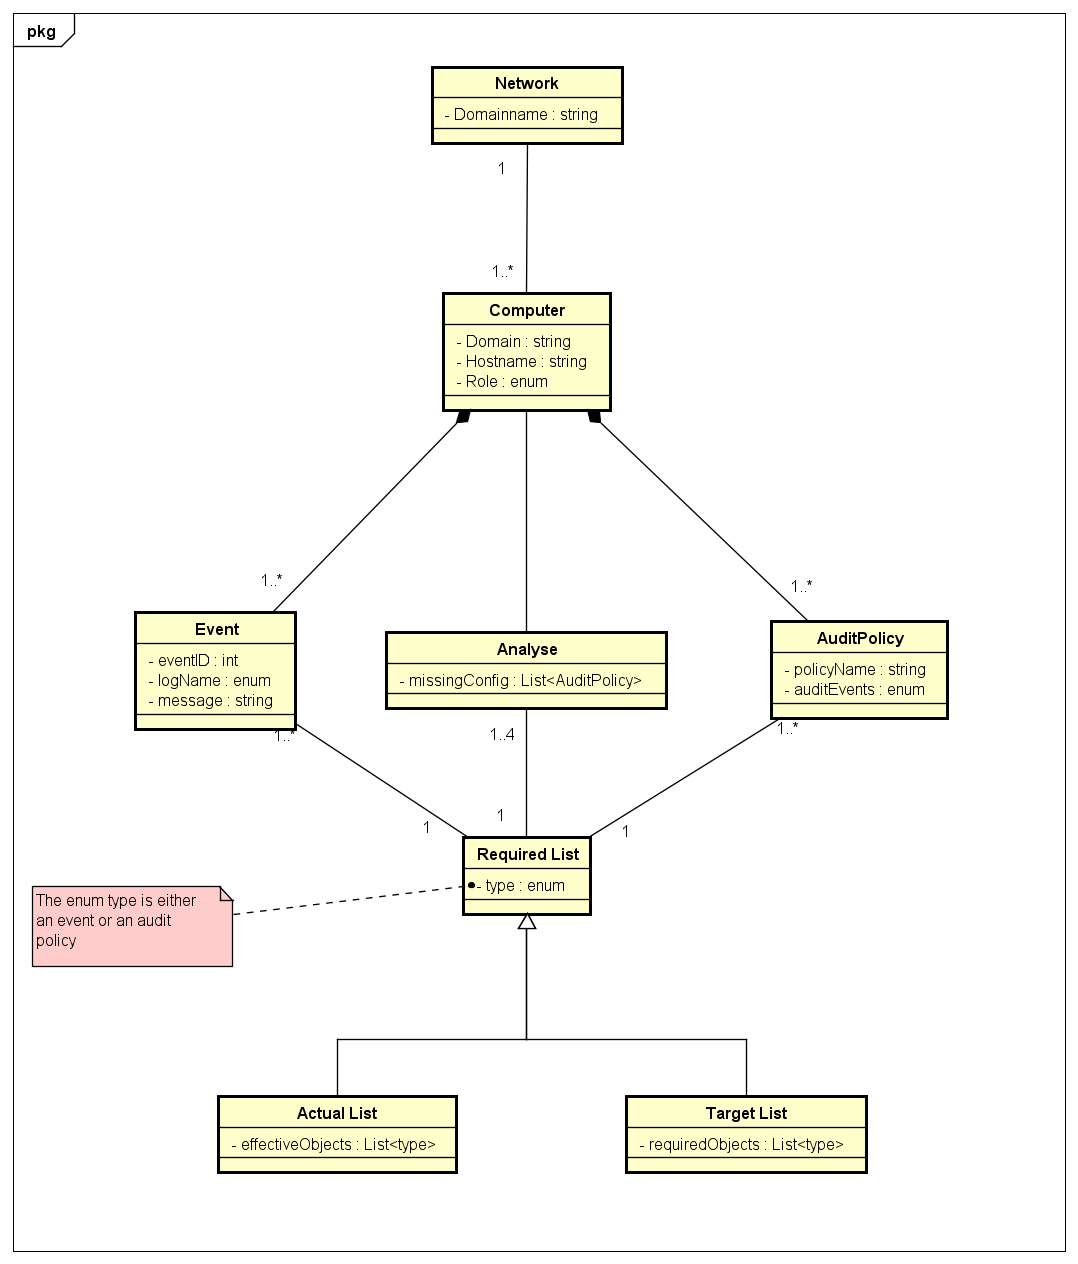
\includegraphics[width=0.95\linewidth]{assets/architecture/DomainModelSRI.png}
    \caption{Domain Model}\label{fig:domainmodel}
\end{figure}

\subsubsection{Network}
The class network depicts the organizations wide network which is used to connect all clients and servers together. In this project the main goal is to locally detect the readiness of the system and not to extend the detection for a system-wide infrastructure. For further development on this project and a system-wide extension, the network is already considered in this domain model.

\subsubsection{Computer}
A computer illustrates either a client like a Windows 10 machine or a server, in particular, a domain controller running on a Windows Server 2016. In principle, however, every Windows computer is represented. A computer is a core component in our project, because the detection is done on a single client or server. 

\subsubsection{Event}
An event represents a single event log entry in simplified form.

\subsubsection{AuditPolicy}\label{DomainModelAuditPolicy}
AuditPolicy displays the individual settings of the audit policies of the group policy, which can be found via \lstinline|gpedit.msc| under ''Computer Configuration > Windows Settings''. However, only the settings under ''Security Settings > Advanced Audit Policy Configuration'' are considered and not the settings under ''Security Settings > Local Policies > Audit Policy''. The reason for this is that Microsoft recommends that only one of the two policies is used:
\begin{quotation}
    \textit{[...] do not use both the basic audit policy settings under Local Policies\textbackslash Audit Policy and the advanced settings under Security Settings\textbackslash Advanced Audit Policy Configuration. Using both basic and advanced audit policy settings can cause unexpected results in audit reporting.} \cite{AdvancedSecurityAuditing}
\end{quotation}
A single audit policy setting represents one or more event IDs logged by this configuration.

\subsubsection{Reference}
\paragraph{ActualList}
The ActualList represents the current state of the system. It reflects the event log IDs that have occurred and the audit policies that have been set.

\paragraph{TargetList}
The TargetList represents either the list of event logs or configured audit policies which must be present for a solid detection of attacks.

\paragraph{DeltaList}
Based on the required lists (audit policies, event logs) as well as the current state of the computer, the DeltaList shows which settings are missing in the audit policies.

\subsection{Conclusion}
The design of the ''System Readiness Inspector'' will be based on the shown tables. The \ref{AttackCategories} \nameref{AttackCategories} and \ref{AuditPolicyPriority} \nameref{AuditPolicyPriority} tables have high priority, they are essential for the evaluation and visualization of the SRI. As seen in \ref{DomainAnalysis} \nameref{DomainAnalysis} the SRI reads out a list of EventLogs and one of the Audit Policies settings. These lists will be compared against a predefined ''correct-list''. Wrong settings will be highlighted.